\defi{4.1} Sean $r,l$ dos rectas con un punto $V$ en común. Sean $\overline{r}$ y $\overline{l}$ dos semirrectas determinadas por $V$ en $r$ y $l$. El par $\{\overline{l}, \overline{r} \}$ es un \textbf{ángulo}. $V$ es el vértice del ángulo y $\overline{l}$ y $\overline{r}$ son los lados del ángulo. El ángulo se designa por $\angle \{\overline{l}, \overline{r} \}$ o, si no hay lugar a confusión, $\angle V$. Así, por ejemplo, dado un triángulo $\triangle PQR$, $\angle P$ es el ángulo formado por $P$ con $[P,Q]$ y $[P,R]$.

\obs{4.4} Si $r = l$, y $\overline{r}_1$ y $\overline{r}_2$ son las semirrectas determinadas por $V$, entonces, en estas circunstancias, el ángulo $\angle\{ \overline{r}_1, \overline{r}_2 \}$ se denomina \textbf{ángulo llano} y $\angle\{ \overline{r}_1, \overline{r}_1 \}$ se denomina \textbf{ángulo nulo}.

\defi{4.5} Un ángulo $\angle \{\overline{l}, \overline{r} \}$ y un ángulo $\angle \{\overline{l}', \overline{r}' \}$ son \textbf{congruentes} si existe una isometría $g$ tal que $g(\{\overline{l}, \overline{r} \}) = \{\overline{l}', \overline{r}'\} $. Todos los ángulos que son congruentes forman una \textbf{clase de congruencia} de ángulos. Empleando la notación de vértices, la congruencia se denota como $\angle A = \angle B$.

\obs{4.6/4.8} Si  $\angle \{\overline{l}, \overline{r} \}$ tiene vértice $V$ y  $\angle \{\overline{l}', \overline{r}' \}$ tiene vértice $V'$, y $g$ es una isometría tal que $g(  \{\overline{l}, \overline{r} \}) =   \{\overline{l}', \overline{r}' \}$, entonces $g(V) = V'$. Asimismo, si existe una isometría $h$ que hace $h(V) = V'$, entonces  $h(  \{\overline{l}, \overline{r} \}) =   \{\overline{l}', \overline{r}' \}$.

\ejem{4.9} Consideramos las rectas $a \neq b$ que cortan en $V$, con sus respectivas semirrectas 
$\overline{a}_1, \overline{a}_2, \overline{b}_1, \overline{b}_2$. Consideramos $\angle \{\overline{a}_1, \overline{b}_1 \}$ y elegimos los puntos $A \in \overline{a}_1, B \in \overline{b}_1$ a igual distancia, $d(V,A) = d(V,B)$. Existe una recta $l \perp r_{AB}$ que pasa por $V$ (\tma{2.25/2.29}, que denominamos \textbf{bisectriz}. La bisectriz $l$ cumple que $\sigma_l(A) = B, \sigma_l(\overline{a}_1) = \overline{b}_1$ y viceversa. Además, si $\overline{l}$ es la semirrecta que corta a $[A,B]$, entonces $\angle \{\overline{a}_1, \overline{l} \} = \angle \{\overline{b}_1, \overline{l} \}$.

\begin{figure}[H]
	\centering
	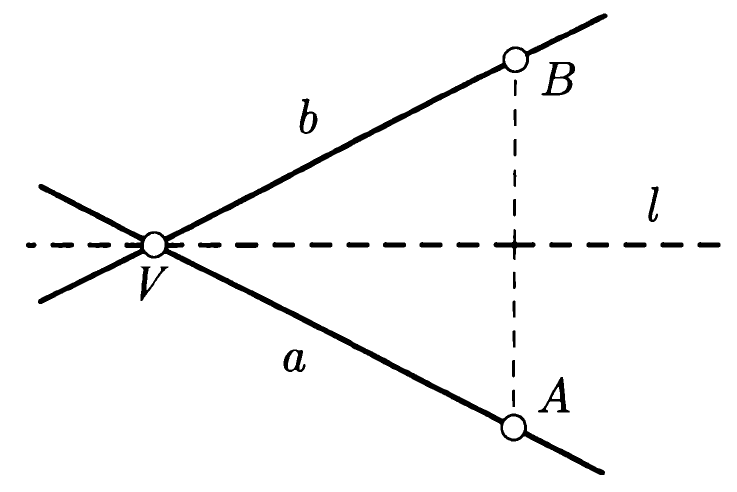
\includegraphics[width=3.5cm]{figuras/4-9.png}
	\vspace{-1em}
\end{figure}

\tma{4.11} Sean $a,b$ que cortan en $V$. El ángulo  $\angle \{\overline{a}_1, \overline{b}_1 \}$ es congruente con  $\angle \{\overline{a}_2, \overline{b}_2 \}$ y se denominan \textbf{ángulos opuestos por el vértice}.

\tma{4.13}/\defi{4.23} Sean $l\perp_V r$ y $l'\perp_{V'}r'$. Entonces  $\angle \{\overline{l}, \overline{r} \}$
y $\angle \{\overline{l}', \overline{r}' \}$ son congruentes. En este caso, los ángulos $\angle \{\overline{l}, \overline{r} \}$
y $\angle \{\overline{l}', \overline{r}' \}$ son \textbf{ángulos rectos}.  Un ángulo es \textbf{agudo} si es menor que un recto, y \textbf{obtuso} si es mayor.
	
\defi{4.15} Si $\angle \{\overline{l}, \overline{r} \}$ no es ni nulo ni llano, y $H_l^1$ es el semiplano que contiene a $\overline{r}$, y $H^1_r$ es el semiplano que contiene a $\overline{l}$, entonces el ángulo $\angle \{\overline{l}, \overline{r} \}$
y $\angle \{\overline{l}, \overline{r} \}$ viene determinado como el conjunto $H^1_l \cap H^1_r$.


\tma{4.18 [De la barra transversal]} Sea   $\angle \{\overline{l}, \overline{r} \}$ con vértice $V$ y sean $L \in \overline{l}, R \in \overline{r}$. Una semirrecta $\overline{s}, V \in \overline{s}$ está dentro de  $\angle \{\overline{l}, \overline{r} \}$ sii corta a $[L,R] - \{L,R\}$.

\begin{figure}[H]
	\centering
	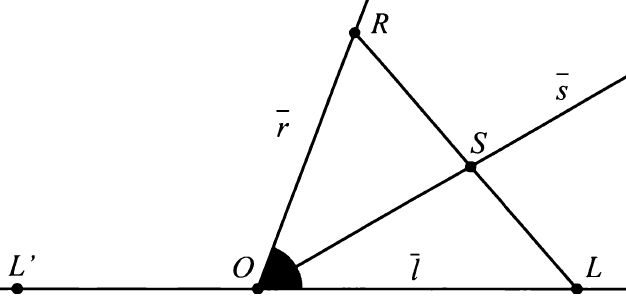
\includegraphics[width=5cm]{figuras/4-18.png}
	\vspace{-1em}
\end{figure}

\defi{4.19 (Comparación de ángulos)} Dados   $\angle \{\overline{a}, \overline{b} \}$ y  $\angle \{\overline{c}, \overline{d} \}$, se dice que $\angle \{\overline{a}, \overline{b} \}$ es menor que $\angle \{\overline{c}, \overline{d} \}$, $\angle \{\overline{a}, \overline{b} \} \prec \angle \{\overline{c}, \overline{d} \}$, si existe una isometría $g$ tal que $g(\overline{a}) = \overline{c}$ y que $g(\overline{b})$ está en el interior de  $\angle \{\overline{c}, \overline{d} \}$

\tma{4.21} Si existen 4 ángulos tales que
 $\angle\{\overline{a}, \overline{b} \} = \angle\{\overline{a}', \overline{b}' \}$ y $\angle\{\overline{c}, \overline{d} \} = \angle\{\overline{c}', \overline{d}' \}$,  y $\angle\{\overline{a}, \overline{b} \} \prec \angle \{\overline{c}, \overline{d} \}$, entonces
$\angle\{\overline{a}', \overline{b}' \} \prec \angle \{\overline{c}', \overline{d}' \}$.

\tma{4.22} Dados  $\angle \{\overline{a}, \overline{b} \}$ y  $\angle \{\overline{c}, \overline{d} \}$, entonces  $\angle \{\overline{a}, \overline{b}\} \prec \angle \{\overline{c}, \overline{d} \}$,  $\angle \{\overline{a}, \overline{b}\} = \angle \{\overline{c}, \overline{d} \}$, o  $\angle \{\overline{a}, \overline{b}\} \succ \angle \{\overline{c}, \overline{d} \}$.

\defi{4.25} Sea  $\angle \{\overline{a}, \overline{c} \}$ con vértice $V$ y $\overline{b}$ una semirrecta en el interior de $\angle \{\overline{a}, \overline{c} \}$. Entonces $\angle \{\overline{a}, \overline{c} \}$ es la \textbf{suma} de $\angle \{\overline{a}, \overline{c} \}$ y $\angle \{\overline{a}, \overline{b} \}$, o $\angle \{\overline{b}, \overline{c} \}=\angle \{\overline{a}, \overline{b} \}+\angle \{\overline{b}, \overline{c} \}$

\defi{4.26} Para tres ángulos $\angle U, \angle V, \angle W$, decimos que $\angle V = \angle U  + \angle W$ si existe una descomposición $\angle V = \angle \{\overline{a}, \overline{c} \}$ ,  $\angle U = \angle \{\overline{a}, \overline{b} \}$ ,  $\angle W = \angle \{\overline{b}, \overline{c} \}$ .

\defi{4.28} Dado $\triangle PQR$, el lado $[R, Q]$ y el ángulo $\angle P$ son \textbf{opuestos}.

\defi{4.29} / \tma{4.30} Un triángulo \textbf{isósceles} tiene dos lados congruentes. Si $\triangle PQR$ es isósceles y $[P,Q]$ es congruente con $[P,R]$, existe una reflexión $\sigma$ tal que $\sigma(P) = P, \sigma(Q) = R, \sigma(R) = Q$, la bisectriz de $\angle P$. Esa isometría que deja invariante el triángulo se denomina \textbf{simetría}.

\defi{4.34} / \tma{4.35} Un triángulo es \textbf{equilátero} si todos sus lados son congruentes. En este caso hay una rotación $\rho$ tal que $\rho(P) = Q, \rho(Q) = R, \rho(R) = P$.

\defi{4.39} / \tma{4.40} Sean $a \parallel b$ y $c$ una recta que corta a $a$ en $A$ y a $b$ en $B$. El par de ángulos $\angle A, \angle B$ de la figura son ángulos \textbf{alternos-internos}.
Los dos ángulos son congruentes.
\begin{figure}[H]
	\centering
	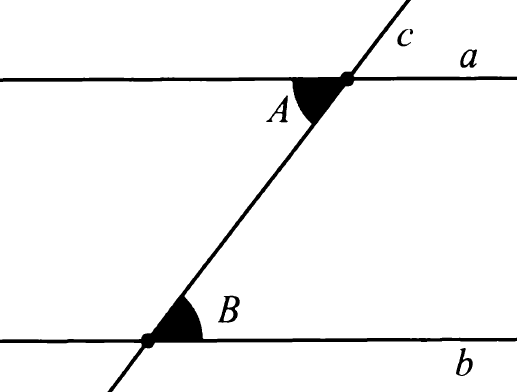
\includegraphics[width=3.5cm]{figuras/4-40.png}
	\vspace{-1em}
\end{figure}

\obligatorio\dem{Sea $m = \m{[A,B]}$. La media vuelta $\sigma_M$ verifica que $\sigma_M(A) = B$ y $\sigma_M(c) = c$. Además, $\sigma_M(a)$ es paralela a $a$ y pasa por $B$, luego por el \axioma{P7}, ha de ser $b$. Por tanto, $\angle\{\overline{a}, \overline{c} \} = \angle\{\overline{b}, \overline{c} \}$ y, por tanto $\angle(A) = \angle(B)$} 

\tma{4.41} La suma de los ángulos de un triángulo es un ángulo llano.

\dem{Si hacemos una recta $p$ paralela a $[Q,R]$ tenemos que $(Q, Q')$ y $(R, R')$ son pares de ángulos internos y la suma  $\angle Q' + \angle P' + \angle R' = \angle Q + \angle P + \angle R$ es un ángulo llano.}
\begin{figure}[H]
	\centering
	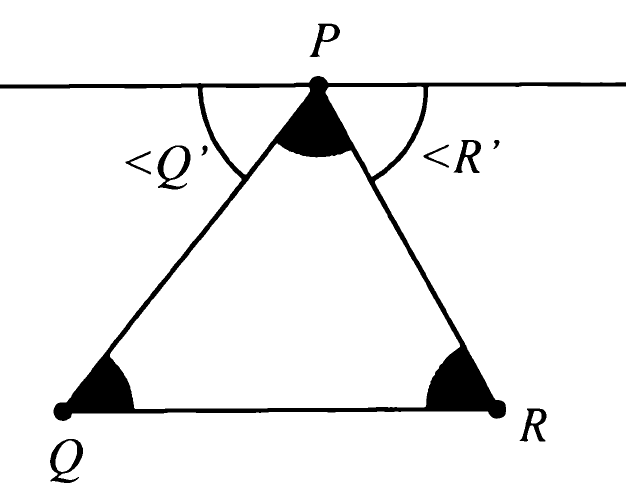
\includegraphics[width=3.5cm]{figuras/4-41.png}
	\vspace{-1em}
\end{figure}

\ej{4.9} Sea $\rho$ una rotación de centro $C$ y sea $t = \triangle\{C, P, \rho(P) \}$. Entonces la clase de congruencia del ángulo $\angle_t C$ se denomina ángulo de rotación $\angle\rho$.

\ej{4.11} Un ángulo orientado es un ángulo donde se fija un orden en sus lados. Dos ángulos orientados $\overrightarrow{\angle}(\overline{r}, \overline{l})$ y  $\overrightarrow{\angle}(\overline{r}', \overline{l}')$ son congruentes si existe una isometría donde $g(\overline{r}) = \overline{r}'$ y $g(\overline{l}) = \overline{l}'$ y se conserva la orientación del plano. Así $\overrightarrow{\angle}(\overline{r}, \overline{l})$ la clase de congruencia con todos los ángulos congruentes.










